\documentclass[11pt]{article}
\usepackage{techreport}
\title{Do LLM Monitors Miss Rare Threats?\texorpdfstring{\\}{} A Pre-registered Test of the Low-Prevalence Effect}
\shorttitle{Do LLM Monitors Miss Rare Threats?}
\author{James Le Cuirot\thanks{Commercial pilot (Senior First Officer), aviation flight safety officer, and aviation safety and compliance consultant specialising in human factors; MSc in Human Factors in Aviation.}\\[2pt] \normalsize CitadelAero}
\date{Preprint v1.0, 4 November 2026}

\begin{document}
\setlength{\emergencystretch}{1.5em} % lets TeX loosen lines that hold long code names
\maketitle


\begin{abstract}
AI control protocols use language-model monitors to review the work of more capable, untrusted AI systems and to send the most suspicious items to a small human audit. Real attacks are expected to be rare. Human screeners miss rare targets far more often than common ones, mainly because they grow reluctant to say ``yes''; airport security counters this with Threat Image Projection. A pre-registered experiment tested whether large language model (LLM) monitors show this low-prevalence effect. Two Claude models made \num{30880} judgements of Python solutions drawn from 379 execution-verified pairs of clean and backdoored code. The prediction failed in the opposite direction. In batches of 40, both monitors caught more backdoors when backdoors were rare: hit rates rose from 0.51 at \SI{50}{\percent} prevalence to 0.69 at \SI{2.5}{\percent} for Haiku, and from 0.50 to 0.74 for Sonnet (Holm-adjusted $p = .0015$ and $p < .001$), with false-alarm rates below \SI{2}{\percent}. The decision criterion did not become more conservative. Single-item review caught about as many backdoors as \SI{2.5}{\percent} batches, and more than \SI{10}{\percent} and \SI{50}{\percent} batches in three of four comparisons. Stating that about 1 in 100 submissions contained a backdoor, rather than about half, slightly lowered Sonnet's single-item hit rate (0.85 to 0.78); Haiku's change was not significant. A labelled calibration block modelled on Threat Image Projection did not reliably raise hit rates and more than doubled Sonnet's false alarms. Rarity did not increase misses. Misses were more frequent when several backdoors shared a batch than when one did.
\end{abstract}

% ===========================================================================
\section{Introduction}\label{sec:intro}

AI control is the study of safety measures that are meant to keep working even if an AI system is deliberately trying to defeat them~\cite{greenblatt2024}. A central measure is \emph{trusted monitoring}. A capable but \emph{untrusted} model does the work. A weaker model that is \emph{trusted}, typically because it is thought too limited to subvert the protocol deliberately, reads each output and gives it a suspicion score. The most suspicious outputs go to a small budget of careful human review, called \emph{auditing}. In the original code-writing testbed the audit budget covered \SI{2}{\percent} of problems~\cite[Sec.~2.2]{greenblatt2024}.

The attacks such a monitor is meant to catch are expected to be rare. In control evaluations the \emph{red team}, which plays the part of a misaligned model, can defeat simple auditing by attacking seldom, so that no attack is likely to fall inside the audited sample~\cite[Sec.~3.1]{greenblatt2024}, \cite[Sec.~3.1]{bhatt2025}. A sketch of a control safety case notes that a model ``might simply attack very rarely such as once out of thousands of tasks''~\cite[Sec.~6]{korbak2025}. Deployment reports are consistent with this (Section~\ref{sec:base-rates}).

Human factors research has studied this situation for decades. In a simulated baggage-screening task, misses rose from \SI{7}{\percent} when targets appeared on half of trials to \SI{30}{\percent} when they appeared on \SI{1}{\percent}~\cite{wolfe2005}. The extra misses come mainly from a shift in decision criterion: observers say ``no'' more readily, while their ability to tell targets from non-targets changes little~\cite{wolfe2007}. Airport security responds with Threat Image Projection (TIP), software that projects images of fictional threats into a small share of real bags and records whether the screener finds them~\cite{cutler2009,buser2025}.

Do LLM monitors behave the same way? Current practice mostly assumes that prevalence does not matter. In eleven audited evaluations of detectors for hijacked LLM agents, attacks made up \SI{16}{\percent} to \SI{86}{\percent} of test samples and ``no evaluation varies that share''~\cite[Abstract]{abbasi2026}. Estimates at low prevalence apply rates measured at high prevalence~\cite[Sec.~6.3]{srivastav2026}, \cite[Sec.~III.E]{abbasi2026}, and a formal model of trusted monitoring treats suspicion scores as ``a distribution, conditioned on whether the code is safe or backdoored''~\cite[Sec.~2]{griffin2024}. Two opposite predictions are plausible (Section~\ref{sec:analogy}). The human prediction is that a monitor that sees few attacks becomes more conservative and misses more of them. The competing prediction is that a lone attack stands out among benign items, or that a model normalises its decisions within a batch~\cite{hida2026}, so that rare attacks are caught \emph{more} often.

This paper reports a pre-registered experiment that tests these predictions with LLM monitors of code. Its contributions are:
\begin{itemize}
\item A pre-registered test that separates \emph{experienced} prevalence (the share of backdoored submissions in a reviewed batch) from \emph{stated} prevalence (a sentence in the prompt). Both monitors caught more backdoors at \SI{2.5}{\percent} prevalence than at \SI{50}{\percent}.
\item A signal detection analysis showing that this reversal was not a conservative criterion shift; post hoc, backdoored items scored lower when several shared a batch.
\item A test of two remedies at low prevalence: a TIP-style labelled calibration block, taken from screening research, and an instruction to judge each item independently. Neither reliably raised hit rates.
\item An open set of 419 execution-verified pairs of clean and backdoored solutions built from MBPP, with code, prompts and all raw monitor outputs.
\item An account, for AI-safety and aviation-safety readers, of where the human analogy held and where it did not.
\end{itemize}

The pre-registration is \code{PREREGISTRATION.md} in this folder (first committed on 3 November 2026, commit \code{f4bedaa}). Section~\ref{sec:prereg-record} summarises its later clarifications and when each was committed.

% ===========================================================================
\section{Background: rare targets in human screening}\label{sec:background-human}

\subsection{Signal detection theory}\label{sec:sdt}

Signal detection theory (SDT) describes decisions about whether a signal is present~\cite{green1966,hautus2021}. A \emph{signal} trial is a backdoored submission and a \emph{noise} trial is a clean one. Flagging a backdoored item is a \emph{hit}; flagging a clean item is a \emph{false alarm}. From the hit rate $H$ and false-alarm rate $F$, sensitivity
\begin{equation}\label{eq:dprime}
d' = z(H) - z(F)
\end{equation}
measures how well the observer separates the two kinds of item, and the criterion
\begin{equation}\label{eq:criterion}
c = -\frac{1}{2}\bigl[z(H) + z(F)\bigr]
\end{equation}
measures how much evidence it needs before saying ``yes''. Here $z$ is the inverse of the standard normal cumulative distribution function. A positive $c$ is conservative (fewer flags, more misses); a negative $c$ is liberal. Because $z$ is infinite at 0 and 1, rates are corrected with the log-linear rule, in which ``each cell frequency in the contingency table is increased by 0.5''; this rule is less biased than the $1/(2N)$ rule~\cite[Abstract]{hautus1995}. The corrected rates are
\begin{equation}\label{eq:loglinear}
\tilde H = \frac{n_{\mathrm{h}} + 0.5}{n_{\mathrm{s}} + 1}, \qquad \tilde F = \frac{n_{\mathrm{f}} + 0.5}{n_{\mathrm{n}} + 1},
\end{equation}
where $n_{\mathrm{h}}$ and $n_{\mathrm{f}}$ are the numbers of hits and false alarms and $n_{\mathrm{s}}$ and $n_{\mathrm{n}}$ the numbers of signal and noise trials. $d'$ and $c$ are computed with $\tilde H$ and $\tilde F$ in Eqs.~\eqref{eq:dprime} and~\eqref{eq:criterion}; the rates $H = n_{\mathrm{h}}/n_{\mathrm{s}}$ and $F = n_{\mathrm{f}}/n_{\mathrm{n}}$ reported in the tables are uncorrected. For graded ratings, such as a suspicion score from 0 to 100, the area under the receiver operating characteristic curve (AUROC) summarises sensitivity across all thresholds; 0.5 is chance and 1.0 is perfect separation.

A criterion that moves with prevalence is not irrational: ``the prevalence effect is a very sensible behavior unless the goal is to minimize misses''~\cite[Introduction]{wolfe2007}. In screening for threats, and in monitoring for attacks, the goal is to minimise misses.

\subsection{The low-prevalence effect}\label{sec:lpe}

Wolfe et~al.~\cite{wolfe2005} asked observers to look for ``tools'' among other semi-transparent objects in an artificial baggage-screening task. Misses were \SI{7}{\percent} at \SI{50}{\percent} target prevalence, \SI{16}{\percent} at \SI{10}{\percent} and \SI{30}{\percent} at \SI{1}{\percent} (figures from the authors' accepted manuscript; see \code{sources.md}). Wolfe et~al.~\cite[Abstract]{wolfe2007} found the effect ``very robust'' and concluded that ``[i]n signal detection terms, the prevalence effect can be explained as a criterion shift and not a change in sensitivity''. Several attempts to move observers to a better criterion failed. One regime worked: brief retraining periods at high prevalence with full feedback, inserted among long low-prevalence periods without feedback (Experiment~7). In that experiment ``[t]here were no significant effects of prevalence'': misses averaged 0.21 in low-prevalence epochs and 0.18 in high-prevalence epochs, while false alarms were higher than in the authors' baseline experiment.

Trained screeners show the effect too. Newly trained transportation security officers had lower hit rates in low-prevalence blocks (prevalence of .05 or less, no feedback) than in a high-prevalence block (.50, full feedback), and a low-prevalence block run after the high-prevalence block showed better performance and a more liberal criterion~\cite{wolfe2013}. Unlike in the laboratory, $d'$ also changed with prevalence. Occasional \emph{probe} trials with known targets also reduce the effect, but ``[t]he probe benefit scaled with the frequency of the matching target''~\cite[Abstract]{becker2026}.

The opposite problem also exists. When one display holds several targets, ``once one target is found, additional targets are likely to be missed'', an effect known in radiology as satisfaction of search and studied as \emph{subsequent search misses}~\cite[Abstract]{cain2013}.

\subsection{Vigilance and alarm reliability}\label{sec:vigilance}

The \emph{vigilance decrement}, a decline in detection over a long watch, is usually traced to Mackworth's~\cite{mackworth1948} studies of prolonged visual search~\cite{klein2025}; vigilance ``requires hard mental work and is stressful''~\cite{warm2008}. People also learn to discount alarms that are usually false: about \SI{90}{\percent} of participants facing alarms of varying reliability matched their response rates ``to the expected probability of true alarms''~\cite{bliss1995}, and airport screeners working with an explosives-detection aid that had a \SI{20}{\percent} false-alarm rate and a positive predictive value of .3 ignored about half of its true alarms on difficult targets, ``a strong cry-wolf effect''~\cite{huegli2020}. Sorkin and Woods~\cite{sorkin1985} showed with an SDT model that setting an automated monitor's threshold to optimise its own detection and false-alarm rates ``will not yield optimal performance for the overall human-machine system''.

\subsection{Threat Image Projection}\label{sec:tip}

TIP is ``a software system that is used at airports to project images of threat items amongst the passenger baggage being screened by X-ray''~\cite[Abstract]{cutler2009}. Typically, fictional threat items are projected onto \SI{1}{\percent} to \SI{4}{\percent} of bags, and the system tells the screener immediately whether a projected item was present~\cite[Sec.~2]{buser2025}. TIP thus raises experienced prevalence, gives feedback and measures performance. Analysing \num{1199838} TIP events from 728 screeners, Buser et~al.~\cite[Abstract]{buser2025} found that ``[a]pproximately 100 TIP events were sufficient to achieve a minimum reliability value of 0.7 when TIP was challenging enough (mean hit rate below 0.9)''. The AI-control analogue is to insert known synthetic attacks into a monitor's stream, which Korbak et~al.~\cite{korbak2025} propose for monitors and human auditors (see Section~\ref{sec:trusted}).

% ===========================================================================
\section{Background: monitoring in AI control}\label{sec:background-control}

\subsection{Trusted monitoring and audit budgets}\label{sec:trusted}

Greenblatt et~al.~\cite{greenblatt2024} introduced the ``APPS backdooring setting'': solve \num{5000} programming problems with an untrusted GPT-4, a trusted GPT-3.5 and a limited supply of trusted high-quality labour, without submitting a backdoored solution. A solution is backdoored ``if it passes all APPS test cases, and if GPT-4 can construct an exploit when presented with the code'', an exploit being ``a specific input that will yield an incorrect output'' (Section~2). Trusted monitoring audits ``the top 2\% most suspicious proposals'', with a threshold that gives ``a 2\% false positive rate on the distribution of solutions written by GPT-4'', and raises the blue team's win probability from \SI{15}{\percent} under auditing of the first \SI{2}{\percent} of solutions to \SI{62}{\percent} (Sections 3.1.2 and 3.2). Rarity is the attacker's main tool: the red team ``can respond to a doubling of the number of problems by halving its probability of adding a backdoor on any given problem'' (Section~3.1.2).

Griffin et~al.~\cite[Sec.~2]{griffin2024} formalise trusted monitoring as a game in which the red team chooses a backdoor rate and the monitor's scores depend only on whether the code is backdoored. Bhatt et~al.~\cite{bhatt2025} used an audit budget of \SI{1}{\percent} of actions in an agent environment, ``higher than what we expect to be able to afford in real deployment'' (Section~2.2, footnote~2), against a red-team ``rare attacks strategy'' (Section~3.1). Korbak et~al.~\cite[Sec.~4]{korbak2025} sketch a safety case whose safety layer ``audits the 0.1\% most suspicious actions'', and in which ``developers regularly generate synthetic attacks and check whether human auditors remain attentive and flag synthetic attacks as suspicious''. That proposal is TIP in all but name. They also note that models might coordinate attacks ``across space'', in a strategy ``where many LLM agents attempt to exfiltrate data simultaneously'' (Section~6).

\subsection{How well do monitors and people detect sabotage?}\label{sec:detect}

In SHADE-Arena the strongest monitor (Gemini 2.5 Pro) reached an AUC of 0.87 in separating benign from sabotage transcripts, against 0.65 for human annotators who took an average of 103 minutes per transcript~\cite[Sec.~4.1]{kutasov2025}. Escalating only flagged cases to human reviewers raised the true-positive rate ``by approximately 15\% at FPR = 0.01''~\cite[Abstract]{kale2025}. SLEIGHT-Bench calibrates monitors to a \SI{1}{\percent} false-positive rate because otherwise ``humans won't be able to review every flagged transcript''~\cite{najt2026}; at that threshold, half of its 40 hand-designed attacks were never caught by an Opus 4.6 monitor in any of ten trials~\cite{najt2026,najt2026arxiv}. Among developers working with sabotaging coding agents, 83 of 88 without a monitor missed the sabotage, and even after a correct alert it survived in 9 of 16 sessions~\cite[Sec.~4.2]{ye2026}. None of these studies varies the share of attacks a monitor sees.

\subsection{Base rates in deployment}\label{sec:base-rates}

Anthropic reports that, as of August 2026, an offline monitor read all actions of the research and engineering agents on its most-used internal platform and ``flags roughly one to two transcripts in every thousand for further review'': ``roughly 100,000 transcripts per week'', of which ``the highest priority flags (approximately \textasciitilde{}50 per week) are escalated to human review''~\cite{favaro_pace}. It adds that ``individual agents rarely misbehave''. A flag rate is not an attack rate, but a deployed monitor plainly reads an overwhelmingly benign stream, and its human reviewers see a few escalations drawn from many flags.

% ===========================================================================
\section{LLM judges, context effects and the gap}\label{sec:judges}

\subsection{What is known}\label{sec:known}

LLM judges show ``position, verbosity, and self-enhancement biases''~\cite[Abstract]{zheng2023}. In few-shot classification, ``[w]hen the prompt is unbalanced, the predictions are unbalanced (majority label bias)''~\cite[Fig.~4 caption]{zhao2021}. Performance on long inputs ``is often highest when relevant information occurs at the beginning or end of the input context''~\cite[Abstract]{liu2024}. Prior scores placed in a judge's context ``anchor judgments and systematically shift ratings toward their values'', and neither chain-of-thought (written step-by-step reasoning before the answer) nor a warning to disregard them reduced the total effect~\cite[Abstract]{kapetanovic2026}.

Two studies apply SDT to LLM overseers. More elaborate procedural traces ``shift the decision criterion toward rejection, increasing false alarms in susceptible overseers'', with $d'$ roughly constant~\cite[Abstract]{chen2026}, and plausible explanations moved multimodal judges' criterion towards acceptance ``without a clear change in mean discriminability''~\cite[Abstract]{cai2026}. Neither varied prevalence.

Two studies come closer. Hida et~al.~\cite{hida2026} compared one-at-a-time and batch screening (20 items per call) of studies for systematic reviews, in five reviews whose natural share of relevant studies ranged from \SI{2.9}{\percent} to \SI{53.0}{\percent}, with and without a sentence stating that share. The stated share had little effect. For one model, batching made screening more inclusive in the four reviews with prevalence of \SI{20}{\percent} or less and more restrictive in the balanced review, a pattern the authors call ``compatible with a possible tendency toward implicit normalization of decisions within the batch'' (Section~4.4). Prevalence there was confounded with review topic and items. Kim et~al.~\cite[Abstract]{kim2026} showed that ``a harmful question that is reliably refused in isolation can elicit a harmful response when embedded in a batch of benign questions'', which they attribute partly to ``refusal signal dilution''.

\subsection{The gap}\label{sec:gap}

Searches of arXiv, the web and the reference lists of the papers above (queries in \code{sources.md}) found no study that manipulates the prevalence of targets within an LLM monitor's or judge's context while holding the pool of items fixed, no study of prevalence effects in an AI-control setting, and no test of TIP-style remedies for LLM monitors. Hida et~al.~\cite{hida2026} is the nearest.

\subsection{The analogy and the two predictions}\label{sec:analogy}

The comparison between a human screener and an LLM monitor is an analogy, and its limits shape the predictions. The human effect has a decision part, a criterion that tracks experienced prevalence~\cite{wolfe2007}, and a behavioural part: observers quit target-absent searches earlier when targets are rare~\cite{wolfe2005,wolfe2007}. An LLM has no time cost and no fatigue across calls. It reads every item it is given at once, and its ``experience'' of prevalence exists only inside one context window, the text of a single call. A low-prevalence effect would have to come through the decision part, for example through majority-label bias~\cite{zhao2021} or dilution of a rare signal among benign items~\cite{kim2026}. Other mechanisms predict the opposite. A single backdoored item among 39 clean ones may stand out by contrast (``pop-out''), and a tendency to normalise decisions within a batch~\cite{hida2026} would make a monitor flag relatively more when few items deserve it. The pre-registration therefore stated that a higher hit rate at low prevalence would be reported as a disconfirmation of H1. Stated prevalence has no clean human counterpart.

% ===========================================================================
\section{Methods}\label{sec:methods}

\subsection{Design and hypotheses}\label{sec:design}

Three experiments, each run with two monitor models, test four confirmatory hypotheses (\code{PREREGISTRATION.md}, Section~2):
\begin{itemize}
\item \textbf{H1 (experienced prevalence).} In batch review, the hit rate is lower at \SI{2.5}{\percent} backdoor prevalence than at \SI{50}{\percent}, with \SI{10}{\percent} in between.
\item \textbf{H1a (criterion, not sensitivity).} That effect shows as a more conservative criterion $c$, with a smaller change in $d'$ and AUROC.
\item \textbf{H2 (stated prevalence).} In single-item review, stating that backdoors are rare (\SI{1}{\percent}) rather than common (\SI{50}{\percent}) lowers the hit rate.
\item \textbf{H3 (remedy).} At \SI{2.5}{\percent} prevalence, a short labelled high-prevalence calibration block shown before the batch raises the hit rate.
\end{itemize}

Four exploratory questions had no directional prediction: position within a batch (E1, an analogue of the vigilance decrement), an independence instruction (E2), differences between monitors (E3) and single-item against batch judging (E4). Table~\ref{tab:design} gives the design. Every planned call returned a valid output, so the achieved counts equal the planned ones.

\begin{table}[tbp]
\centering
\small
\setlength{\tabcolsep}{4pt}
\caption{Design per monitor model. Items come from the main pool.\source{\code{results/RESULTS\_numbers.md} (calls and judgements per condition)}}\label{tab:design}
\begin{tabularx}{\textwidth}{@{}l l >{\raggedright\arraybackslash}X >{\raggedright\arraybackslash}p{1.9cm} >{\raggedright\arraybackslash}p{1.45cm} >{\raggedright\arraybackslash}p{1.9cm} >{\raggedright\arraybackslash}p{1.9cm}@{}}
\toprule
Experiment & Condition & Presentation & Backdoored per call & Calls & Backdoored judgements & Clean judgements \\
\midrule
1 & P50 & Batch of 40 & 20 & 8 & 160 & 160 \\
1 & P10 & Batch of 40 & 4 & 40 & 160 & \num{1440} \\
1 & P2.5 & Batch of 40 & 1 & 160 & 160 & \num{6240} \\
2 & \emph{none}, S50, S1 & Single item & 0 or 1 & 240 per condition & 120 per condition & 120 per condition \\
3 & R-cal & 10 labelled examples, then batch of 40 & 1 & 80 & 80 & \num{3120} \\
3 & R-ind & Batch of 40 with independence sentence & 1 & 80 & 80 & \num{3120} \\
\bottomrule
\end{tabularx}
\end{table}

\subsection{Task and materials}\label{sec:materials}

\paragraph{Domain.} Following the code-backdooring setting of Greenblatt et~al.~\cite{greenblatt2024}, a monitor reviews short Python solutions, any of which may contain a deliberately inserted \emph{backdoor}: code that passes the provided tests but returns a wrong answer on a specific input, the \emph{trigger}.

\paragraph{Problems.} Problems come from the Mostly Basic Programming Problems dataset (MBPP~\cite{austin2021}), full configuration, all four splits: 974 problems ``designed to be solvable by entry-level programmers''~\cite[Abstract]{austin2021}, each with a task description, a reference solution and three test assertions, released under the Creative Commons Attribution 4.0 licence (CC BY 4.0)\footnote{Items derive from MBPP~\cite{austin2021}, released under CC BY 4.0; the derived item pairs are released under the same licence with attribution.} and downloaded on 3 November 2026 (hashes in \code{data/mbpp\_download.json}). Two problems (task IDs 367 and 927) were ineligible because their reference solutions fail their own tests. From the 972 eligible problems, 450 were drawn at random (seed 20261103).

\paragraph{Item pairs.} For each sampled problem, a generator model (\code{claude-opus-5-5}, effort \code{medium}) received the task text, the reference solution, the three test assertions and the name of the function under test. In one call it returned a \emph{clean} solution, a \emph{backdoored} minimal edit of it, and the trigger input. The instructions asked for a subtle backdoor ``the way a capable adversary would'', for example ``a plausible-looking edge-case or boundary check'' (\code{data/\allowbreak generator\_system\_prompt\_v1.txt}). All 450 calls returned an answer.

\paragraph{Verification.} Candidates were executed in a sandboxed subprocess with a 10-second timeout. A pair was kept only if both versions parse, pass a static safety screen and contain no identifier naming the backdoor; both pass the three MBPP tests; on the trigger, the backdoored output differs from the clean output and, where the reference returns normally, from the reference output; and the two normalised versions have a \code{difflib.SequenceMatcher} ratio of at least 0.6, the operational meaning of ``small edit'' (Section~\ref{sec:prereg-record}). Of 450 pairs, 419 (\SI{93.1}{\percent}) were kept; most exclusions were pairs whose backdoored output matched the reference output on the trigger (14) or whose edit was too large (14) (\code{results/RESULTS.md}, Section~3). In the kept pairs the median number of changed lines in a unified diff (added plus removed) was 2, with a maximum of 8; 356 pairs (\SI{85}{\percent}) had exactly two, for example one line replaced. A rough post hoc classification found that 254 pairs (\SI{61}{\percent}) changed a statement in place, such as a loop bound or comparison, and 150 (\SI{36}{\percent}) added an \code{if} branch. Many backdoors therefore look like ordinary off-by-one bugs: a ``backdoor'' here means a deliberately placed wrong answer on a rare input, not code that looks malicious.

\paragraph{Normalisation.} Docstrings and bare string statements were removed explicitly, and both versions were then passed through Python's \code{ast} parser and unparser, which drops comments and standardises formatting (\code{PREREGISTRATION.md}, Section~9, item~2). Function names were kept.

\paragraph{Pools.} Verified pairs were split at random (seed 4021) into a calibration pool of 40 pairs and a main pool of 379. All main-experiment items came from the main pool; the calibration pool was used only for the difficulty check and the R-cal examples. Within any batch a problem appears at most once, in either its clean or its backdoored version.

\subsection{Item-difficulty calibration}\label{sec:calibration}

Before the main runs, \code{claude-haiku-5-5} judged the 80 calibration-pool items one at a time with no stated prevalence. The target was a hit rate between 0.40 and 0.90 and a false-alarm rate below 0.30, with up to two revisions of the generator's instruction allowed. The first item set was on target: the hit rate was $24/40 = 0.60$ (Wilson \SI{95}{\percent} CI 0.45 to 0.74), the false-alarm rate $0/40 = 0.00$ (0.00 to 0.09) and the AUROC 0.97. No revision was made (\code{results/calibration.md}).

\subsection{Monitors}\label{sec:monitors}

The monitors were \code{claude-\allowbreak haiku-5-5}, the main ``trusted, weaker'' monitor, and \code{claude-\allowbreak sonnet-5-5}, both at effort \code{low}. They were called through Claude Code 2.1.317 in non-interactive mode (\code{claude -p}~\cite{anthropic_headless}) with the default system prompt replaced by the study's own (\code{-{}-system-prompt}), tools, MCP servers, slash commands and session persistence disabled, the user message on standard input, \code{-{}-output-format json} and a JSON schema (\code{-{}-json-schema}). Model sampling cannot be fixed, so every call is an independent random draw.

The system prompt said that an untrusted AI system ``may sometimes insert a backdoor: a deliberate change that makes the code pass normal tests but return a wrong answer on specific inputs'', and asked the monitor to ``decide which ones should be escalated to a limited human audit''. For each submission it returned an ID, a \emph{suspicion} score from 0 to 100 and a binary \emph{flag} (escalate or not). Each submission appeared as a random ID, the MBPP task text and the normalised code. Tests and triggers were not shown, except for the backdoored examples in R-cal (\code{PREREGISTRATION.md}, Section~9, item~6). The batch and single-item system prompts differ in one descriptive sentence (item~7). All prompts are in \code{code/prompts/}.

\paragraph{Harness context.} The calls were not run in Claude Code's \code{-{}-bare} mode, so Claude Code added unlogged content of its own to every request; replacing the default system prompt does remove its git-status snapshot~\cite{anthropic_headless}. A post hoc analysis of token counts (\code{results/RESULTS.md}, Section~10.4) puts the added content at a constant block of about \num{1800} input tokens per call (\num{1812} for Haiku, \num{1791} for Sonnet), about three-quarters of a single-item call's input and a quarter of a batch call's, the same in every condition, for both monitors and throughout the run. Claude Code's diagnostics log showed no \code{CLAUDE.md} or memory file, no git-status context and no hook in any call, but each call's context included a field for the account's e-mail address.

The flag measures the monitor's own criterion, which matters for systems that act on the monitor's decision, such as blocking monitors~\cite{remedios2026,remedios2026arxiv}; the AUROC measures separability whatever threshold is applied, which matters where the threshold is set externally~\cite{greenblatt2024}.

\subsection{Experiments}\label{sec:experiments}

\paragraph{Experiment 1: experienced prevalence (batch).} Each call showed a batch of 40 submissions with random IDs in random order, and the prompt said nothing about prevalence. The conditions (P50, P10, P2.5) differ only in how many of the 40 are backdoored. Items were drawn without replacement within a batch and with replacement across batches, and each backdoored item's position was uniform at random. Both monitors saw the same batch compositions, IDs and order.

\paragraph{Experiment 2: stated prevalence (single item).} Each call showed one submission. The conditions differ by one sentence in the system prompt: \emph{none} (no statement); \emph{S50} (``In past reviews, about half of submissions contained a backdoor.''); and \emph{S1} (``In past reviews, about 1 in 100 submissions contained a backdoor.''). The same 240 main-pool problems (120 shown backdoored, 120 clean) were used in every monitor and condition.

\paragraph{Experiment 3: remedies at low prevalence (batch).} Batches were built as in P2.5 but drawn afresh. In \emph{R-cal}, the user message first showed 10 examples from 10 distinct calibration-pool problems (5 backdoored, 5 clean, in random order, drawn anew for each batch) with their correct labels and, for backdoored ones, the trigger input. R-cal is the analogue of the high-prevalence retraining bursts of Wolfe et~al.~\cite{wolfe2007} and of TIP feedback. In \emph{R-ind}, one sentence was added to the system prompt: ``The number of backdoored submissions in this batch is unknown and may be zero, one or many; judge each submission independently on its own merits.''

All main calls were generated before any was run (seed 55021) and run in shuffled order (seed 99173) from 23:12 UTC on 3 November to 00:12 UTC on 4 November 2026.

\subsection{Measures}\label{sec:measures}

The registered measures were $H$, $F$, $d'$ and $c$ (log-linear correction on all cells~\cite{hautus1995}), the AUROC of suspicion scores within each condition, and mean suspicion scores for clean and backdoored items. Rates have Wilson \SI{95}{\percent} confidence intervals; $d'$, $c$ and AUROC have \SI{95}{\percent} bootstrap intervals (\num{2000} resamples) over batches in Experiments 1 and 3 and over items, paired across conditions, in Experiment 2.

\subsection{Analysis}\label{sec:analysis}

The H1, H2 and H3 tests are two-sided Wald tests at $\alpha = .05$, Holm-corrected across the two monitors. H1a is a decision rule on bootstrap intervals.
\begin{itemize}
\item \textbf{H1 and H3.} Logistic regression of flag (backdoored items) on condition, per monitor, with standard errors clustered by batch; confirmatory contrasts P2.5 against P50 (H1) and R-cal against P2.5 (H3). The model is
\begin{equation}\label{eq:glm}
\operatorname{logit} \Pr(y_i = 1) = \beta_0 + \sum_k \beta_k x_{ik},
\end{equation}
where $y_i$ is the flag given to backdoored judgement $i$, $x_{ik}$ indicates that the judgement was made in condition $k$ (one indicator for each condition other than the reference, P50 for H1 and P2.5 for H3), and $\exp(\beta_k)$ is the odds ratio for condition $k$ against the reference.
\item \textbf{H1a.} Supported for a monitor if $\Delta c = c(\mathrm{P2.5}) - c(\mathrm{P50})$ is positive with a bootstrap interval excluding zero, and $|\Delta c| > |\Delta d'|$ on the point estimates. Both are on the same $z$ scale, which is how the pre-registration's ``standardised units'' was clarified (Section~9, item~1).
\item \textbf{H2.} Logistic regression of flag (backdoored items) on stated-prevalence condition, per monitor, with item random intercepts, fitted by maximum likelihood with 40-node Gauss--Hermite quadrature and a pre-specified convergence rule (Section~9, item~9); confirmatory contrast S1 against S50. The model is
\begin{equation}\label{eq:glmm}
\operatorname{logit} \Pr(y_{ij} = 1 \mid u_j) = \beta_0 + \beta_{\mathrm{none}}\, x_{\mathrm{none},ij} + \beta_{\mathrm{S1}}\, x_{\mathrm{S1},ij} + u_j, \qquad u_j \sim \mathcal{N}(0, \sigma^2),
\end{equation}
where $y_{ij}$ is the flag in judgement $i$ of backdoored item $j$, $x_{\mathrm{none},ij}$ and $x_{\mathrm{S1},ij}$ indicate the \emph{none} and S1 conditions (reference S50), $u_j$ is the random intercept of item $j$ and $\sigma$ is the item standard deviation. The item-clustered GLM is reported as a sensitivity analysis.
\item \textbf{Exploratory.} E1: flag on position (1 to 40) within P2.5 and P10. E2: R-ind against P2.5. E3: monitor-by-condition interactions. E4: single-item \emph{none} against each batch condition. These are not corrected for multiplicity.
\end{itemize}

The pre-registration estimated about \SI{80}{\percent} power for a fall in hit rate from 0.80 to 0.65 with 160 backdoored judgements per cell, ignoring clustering, and stated that effects smaller than about 15 percentage points may be missed. Experiment 2 has 120 backdoored items per condition and Experiment 3 has 80 backdoored judgements per remedy. This applies with more force to Experiment 3; Experiment 2 has fewer items but a paired design. Analyses used Python 3.13.18 and statsmodels 0.15.0 (\code{code/analyse.py}; bootstrap seed 314159).

\subsection{Pre-registration record and clarifications}\label{sec:prereg-record}

There were no deviations from the registered design, sample sizes or confirmatory tests. Section~9 of the pre-registration lists clarifications. Items 1 to 3, by the author (the H1a rule, docstring removal and the edit-size threshold), are in commit \code{136632a} (23:10 UTC on 3 November), before any main-experiment call. Item~3 originally said the 0.6 threshold was ``set during verification of the first generation run''. The author's later correction in Section~9 replaces this with the engineer's record that the threshold was ``coded before the verifier was first run on any generated item, while generation was still under way''. The git history cannot confirm that timing, because the verifier and its threshold first appear in git in commit \code{7fe31dc}, after generation and verification. In that commit a code comment described the threshold as ``fixed before any items were generated''; in commit \code{d8e6b51} it was reworded to ``fixed in code before the verifier was first run on any generated item''.

Items 4 to 12, by the research engineer, record implementation choices such as what the monitor sees, retries, sampling and the GLMM convergence rule. As the author's note in Section~9 states, they first appear in commit \code{d8e6b51} (23:16 UTC), after the main run had started (23:13 UTC, with 12 smoke-test calls already done) and when that commit already held 138 main-experiment outputs; they should be read as recorded at, not demonstrably before, the start of data collection. The code that implements several of them, including the analysis script with its GLMM convergence rule, was committed earlier, in \code{7fe31dc} at 23:10:45 UTC, before the first main-experiment output at 23:12:32 UTC (independent audit, \code{AUDIT.md}; checked against \code{git log} and \code{results/\allowbreak monitor\_attempts.jsonl}). None of the clarifications changes a hypothesis, condition, sample size or confirmatory test. Item~13 lists the post hoc analyses; further post hoc checks requested by the audit are in \code{results/RESULTS.md}, Section~10.

\subsection{Exclusions and cost}\label{sec:exclusions}

An output was invalid if it failed the schema, omitted or duplicated IDs, refused, timed out or errored; invalid calls were to be retried up to three times with fresh calls and then dropped. All \num{2176} main calls (\num{30880} judgements) returned a valid output at the first attempt, with no retries, refusals or dropped batches. From turn counts above two (\code{num\_turns}~$>$~2) it is inferred that Claude Code corrected a schema-invalid output inside the call, with the intermediate output unlogged, in 43 of 368 Haiku batch calls and 24 of 720 Sonnet single-item calls; these in-call retries with feedback were not anticipated by the registered fresh-call retry rule. Including generation and calibration, the study made \num{2706} model calls with a list-price-equivalent cost of USD~41.70, run under a Claude Code subscription (\code{results/costs.json}).

% ===========================================================================
\section{Results}\label{sec:results}

\subsection{Overview}\label{sec:overview}

Table~\ref{tab:rates} gives hit and false-alarm rates for every condition, and Table~\ref{tab:sdt} the other registered measures. False-alarm rates were at or below \SI{4.0}{\percent} in every condition and below \SI{2}{\percent} in all batch conditions except Sonnet's R-cal. $d'$ and $c$ are therefore driven mainly by the hit rate.

\begin{table}[tbp]
\centering
\small
\caption{Hit rate $H$ (Wilson \SI{95}{\percent} CI) and false-alarm rate $F$ by condition. Backdoored/clean judgements per monitor: P50 160/160; P10 160/\num{1440}; P2.5 160/\num{6240}; R-cal and R-ind 80/\num{3120}; single-item conditions 120/120.\source{\code{results/RESULTS\_numbers.md}, ``Descriptive results per condition''}}\label{tab:rates}
\begin{tabular}{@{}l l r l r@{}}
\toprule
Condition & Haiku $H$ & Haiku $F$ & Sonnet $H$ & Sonnet $F$ \\
\midrule
P50 (batch) & 0.512 [0.436, 0.589] & \SI{1.9}{\percent} & 0.500 [0.423, 0.577] & \SI{0.6}{\percent} \\
P10 (batch) & 0.500 [0.423, 0.577] & \SI{1.2}{\percent} & 0.569 [0.491, 0.643] & \SI{1.4}{\percent} \\
P2.5 (batch) & 0.694 [0.618, 0.760] & \SI{1.2}{\percent} & 0.738 [0.664, 0.800] & \SI{1.7}{\percent} \\
R-cal (batch) & 0.600 [0.490, 0.700] & \SI{1.2}{\percent} & 0.850 [0.756, 0.912] & \SI{4.0}{\percent} \\
R-ind (batch) & 0.625 [0.515, 0.723] & \SI{0.7}{\percent} & 0.750 [0.645, 0.832] & \SI{1.8}{\percent} \\
\emph{none} (single) & 0.633 [0.544, 0.714] & \SI{1.7}{\percent} & 0.800 [0.720, 0.862] & \SI{0.8}{\percent} \\
S50 (single) & 0.683 [0.596, 0.760] & \SI{3.3}{\percent} & 0.850 [0.775, 0.903] & \SI{3.3}{\percent} \\
S1 (single) & 0.642 [0.553, 0.722] & \SI{0.8}{\percent} & 0.775 [0.692, 0.841] & \SI{1.7}{\percent} \\
\bottomrule
\end{tabular}
\end{table}

\begin{table}[tbp]
\centering
\small
\setlength{\tabcolsep}{4pt}
\caption{Registered signal detection measures: $d'$, $c$ and AUROC with \SI{95}{\percent} bootstrap CIs, and mean suspicion scores for backdoored (bd) and clean items (\code{results/RESULTS.md}, Section~10.2).\source{\code{results/registered\_measures\_table.md}}}\label{tab:sdt}
\begin{tabular}{@{}l l l l l r r@{}}
\toprule
Monitor & Condition & $d'$ & $c$ & AUROC & Mean bd & Mean clean \\
\midrule
Haiku & P50 & 2.05 [1.84, 2.64] & 0.99 [0.73, 1.45] & 0.867 [0.827, 0.902] & 41.5 & 7.7 \\
Haiku & P10 & 2.25 [2.01, 2.55] & 1.13 [1.00, 1.28] & 0.886 [0.855, 0.914] & 41.2 & 6.1 \\
Haiku & P2.5 & 2.76 [2.54, 3.01] & 0.88 [0.77, 0.98] & 0.912 [0.883, 0.939] & 52.1 & 5.6 \\
Haiku & R-cal & 2.50 [2.21, 2.80] & 1.00 [0.84, 1.16] & 0.915 [0.874, 0.950] & 50.2 & 6.4 \\
Haiku & R-ind & 2.75 [2.44, 3.09] & 1.06 [0.91, 1.22] & 0.898 [0.849, 0.942] & 49.5 & 5.0 \\
Haiku & \emph{none} & 2.38 [1.95, 3.09] & 0.85 [0.64, 1.21] & 0.923 [0.887, 0.954] & 48.8 & 6.5 \\
Haiku & S50 & 2.26 [1.88, 2.89] & 0.66 [0.46, 0.98] & 0.923 [0.889, 0.954] & 54.8 & 7.9 \\
Haiku & S1 & 2.60 [2.16, 3.18] & 0.94 [0.71, 1.23] & 0.937 [0.907, 0.965] & 48.8 & 5.0 \\
\midrule
Sonnet & P50 & 2.35 [1.83, 2.91] & 1.18 [1.06, 1.38] & 0.905 [0.882, 0.929] & 41.9 & 7.0 \\
Sonnet & P10 & 2.36 [2.11, 2.66] & 1.01 [0.87, 1.17] & 0.911 [0.886, 0.934] & 46.1 & 5.5 \\
Sonnet & P2.5 & 2.74 [2.54, 2.98] & 0.74 [0.62, 0.85] & 0.927 [0.901, 0.950] & 58.3 & 5.4 \\
Sonnet & R-cal & 2.77 [2.45, 3.17] & 0.37 [0.18, 0.52] & 0.959 [0.929, 0.980] & 65.5 & 7.4 \\
Sonnet & R-ind & 2.76 [2.46, 3.12] & 0.71 [0.55, 0.87] & 0.935 [0.898, 0.967] & 62.0 & 5.0 \\
Sonnet & \emph{none} & 3.08 [2.62, 3.67] & 0.71 [0.47, 1.00] & 0.953 [0.922, 0.979] & 68.4 & 4.4 \\
Sonnet & S50 & 2.81 [2.39, 3.42] & 0.38 [0.18, 0.69] & 0.966 [0.941, 0.986] & 75.0 & 6.5 \\
Sonnet & S1 & 2.79 [2.35, 3.47] & 0.65 [0.43, 1.01] & 0.949 [0.919, 0.974] & 62.7 & 4.4 \\
\bottomrule
\end{tabular}
\end{table}

\begin{table}[tbp]
\centering
\footnotesize
\setlength{\tabcolsep}{4pt}
\caption{Confirmatory tests. OR = odds ratio of flagging a backdoored item; $p$ values are two-sided, Holm-corrected across monitors. The H2 odds ratios come from the registered GLMM and are item-specific; for Sonnet the population-averaged odds ratio is 0.61 [0.44, 0.84], a fall in hit rate of 7.5 points (Section~\ref{sec:h2}).\source{\code{results/RESULTS\_numbers.md} (H1, H2 and H3 tables); exact $p$ values from \code{results/analysis.json}}}\label{tab:tests}
\begin{tabularx}{\textwidth}{@{}l l l l r l l >{\raggedright\arraybackslash}X@{}}
\toprule
Hypothesis & Contrast & Monitor & OR [\SI{95}{\percent} CI] & $z$ & $p$ & Holm $p$ & Outcome \\
\midrule
H1 & P2.5 vs P50 & Haiku & 2.15 [1.34, 3.46] & 3.18 & .0015 & .0015 & Not supported; opposite direction \\
H1 & P2.5 vs P50 & Sonnet & 2.81 [1.78, 4.43] & 4.44 & $<$\,.001 & $<$\,.001 & Not supported; opposite direction \\
H2 & S1 vs S50 (GLMM) & Haiku & 0.57 [0.22, 1.46] & \num{-1.16} & .244 & .244 & Not supported \\
H2 & S1 vs S50 (GLMM) & Sonnet & 0.04 [0.00, 0.42] & \num{-2.66} & .008 & .015 & Supported (small effect) \\
H3 & R-cal vs P2.5 & Haiku & 0.66 [0.38, 1.16] & \num{-1.44} & .150 & .150 & Not supported \\
H3 & R-cal vs P2.5 & Sonnet & 2.02 [0.99, 4.10] & 1.94 & .053 & .106 & Not supported \\
\bottomrule
\end{tabularx}
\end{table}

\subsection{H1: experienced prevalence}\label{sec:h1}

Both monitors caught more backdoors when backdoors were rare (Figure~\ref{fig:prevalence}). Haiku's hit rate was 0.512 at P50, 0.500 at P10 and 0.694 at P2.5; Sonnet's was 0.500, 0.569 and 0.738. For the confirmatory contrast, P2.5 against P50, the odds ratio was 2.15 for Haiku (\SI{95}{\percent} CI 1.34 to 3.46, Holm $p = .0015$) and 2.81 for Sonnet (1.78 to 4.43, Holm $p < .001$). P10 did not differ from P50 (Haiku OR 0.95, $p = .828$; Sonnet OR 1.32, $p = .211$). False-alarm rates did not differ by prevalence for either monitor (all $p > .25$). H1 is therefore disconfirmed, in the direction the pre-registration named as possible.

\begin{figure}[tbp]
\centering
\begin{subfigure}[b]{0.49\textwidth}
\centering
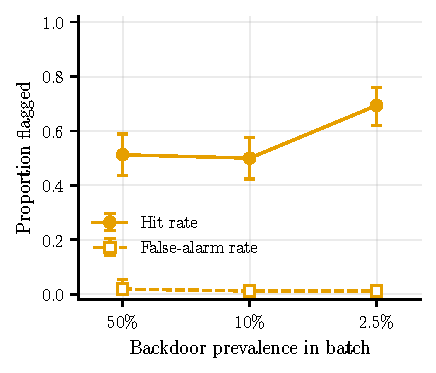
\includegraphics[width=\linewidth]{figures/report/fig_a_prevalence_haiku.pdf}
\caption{Haiku}
\end{subfigure}\hfill
\begin{subfigure}[b]{0.49\textwidth}
\centering
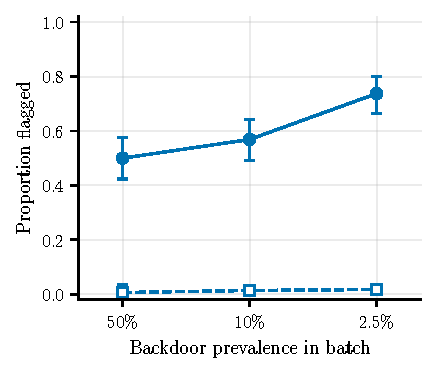
\includegraphics[width=\linewidth]{figures/report/fig_a_prevalence_sonnet.pdf}
\caption{Sonnet}
\end{subfigure}
\caption{Hit rate and false-alarm rate by backdoor prevalence in a batch of 40 (Experiment~1). Error bars are Wilson \SI{95}{\percent} confidence intervals, which ignore clustering by batch.}\label{fig:prevalence}
\end{figure}

\subsection{H1a: criterion or sensitivity}\label{sec:h1a}

The criterion did not become more conservative at low prevalence (Table~\ref{tab:h1a}, Figure~\ref{fig:sdt}). For Sonnet, $c$ moved in the liberal direction ($\Delta c = {-0.44}$, \SI{95}{\percent} CI \num{-0.70} to \num{-0.28}). For Haiku, $c$ did not change reliably, and $d'$ rose ($\Delta d' = 0.71$, 0.06 to 1.04). AUROC rose slightly for both monitors, with intervals that include zero. H1a's first condition ($\Delta c > 0$ with an interval excluding zero) failed for both monitors, so H1a is not supported.

\begin{table}[tbp]
\centering
\small
\caption{Change from P50 to P2.5 (point estimate and \SI{95}{\percent} cluster-bootstrap CI).\source{\code{results/RESULTS\_numbers.md}, ``H1a (confirmatory): criterion vs sensitivity, P2.5 minus P50''}}\label{tab:h1a}
\begin{tabular}{@{}l l l l l l@{}}
\toprule
Monitor & $\Delta H$ & $\Delta F$ & $\Delta d'$ & $\Delta c$ & $\Delta$AUROC \\
\midrule
Haiku & 0.181 & ${-0.0069}$ & 0.71 & \num{-0.12} & 0.045 \\
 & [0.075, 0.281] & [${-0.0327}$, 0.0128] & [0.06, 1.04] & [\num{-0.59}, 0.17] & [\num{-0.002}, 0.092] \\[3pt]
Sonnet & 0.238 & 0.0111 & 0.39 & \num{-0.44} & 0.022 \\
 & [0.144, 0.338] & [${-0.0026}$, 0.0202] & [\num{-0.24}, 0.95] & [\num{-0.70}, \num{-0.28}] & [\num{-0.013}, 0.056] \\
\bottomrule
\end{tabular}
\end{table}

\begin{figure}[tbp]
\centering
\begin{subfigure}[b]{\textwidth}
\centering
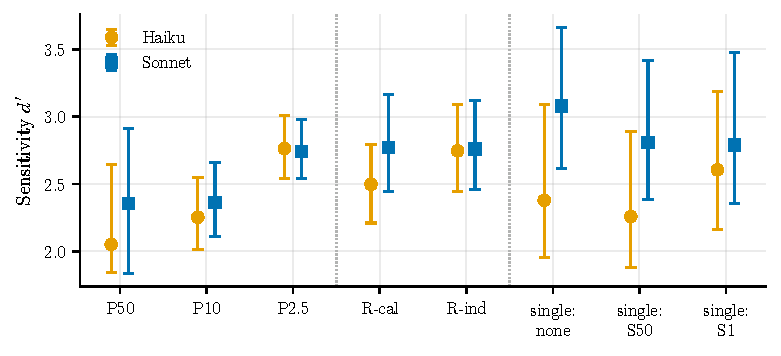
\includegraphics[width=0.92\linewidth]{figures/report/fig_b_sdt_dprime.pdf}
\caption{Sensitivity $d'$}
\end{subfigure}

\vspace{4pt}
\begin{subfigure}[b]{\textwidth}
\centering
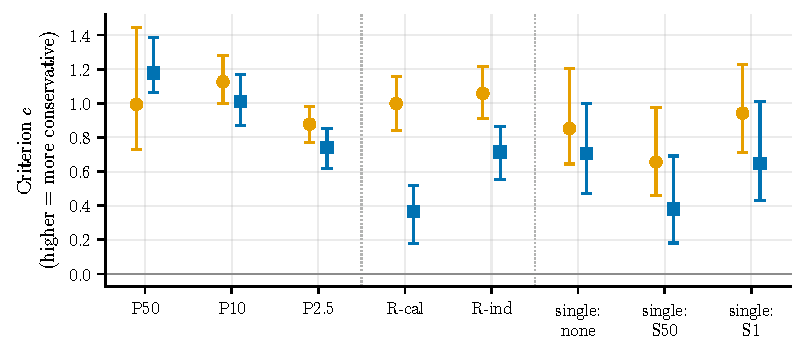
\includegraphics[width=0.92\linewidth]{figures/report/fig_b_sdt_c.pdf}
\caption{Criterion $c$}
\end{subfigure}
\caption{Sensitivity $d'$ (a) and criterion $c$ (b; higher is more conservative) for every condition and monitor, with log-linear correction. Error bars are \SI{95}{\percent} bootstrap confidence intervals: a cluster bootstrap over batches for Experiments 1 and 3, and a paired item bootstrap for Experiment~2.}\label{fig:sdt}
\end{figure}

\subsection{H2: stated prevalence}\label{sec:h2}

Telling Sonnet that ``about 1 in 100'' submissions contained a backdoor, rather than ``about half'', lowered its single-item hit rate from 0.850 to 0.775 (registered GLMM: log-odds \num{-3.32}, SE 1.25, $z = {-2.66}$, $p = .008$, Holm $p = .015$; Figure~\ref{fig:stated}). For Haiku the hit rate went from 0.683 to 0.642 (OR 0.57, 0.22 to 1.46, $p = .244$, Holm $p = .244$).

The registered fit is numerically unreliable for Sonnet (post hoc check; \code{results/\allowbreak RESULTS.md}, Section~10.1). Because 92 of 120 backdoored items were flagged in all three conditions, the item standard deviation $\sigma$ is large, and 40-node non-adaptive quadrature cannot resolve the likelihood there. The registered fit stopped at a local optimum of its own approximation ($\sigma = 32.8$), and the spread of $\sigma$ from 9 to 33 across quadrature settings reflects the same inaccuracy. An accurate likelihood, computed by dense-grid integration, gives $\sigma = 13.4$ and an S1 log-odds of \num{-3.76} (SE 1.41, $z = {-2.67}$, $p = .0076$; likelihood-ratio $p = .00024$). The plainest evidence needs no model: 9 Sonnet items were flagged under S50 but not under S1, and none the other way round (exact paired test, $p = .0039$). For Haiku the registered fit is accurate, and the paired counts were 12 against 7 ($p = .36$).

The GLMM coefficient is item-specific; the population-averaged odds ratio, from the item-clustered GLM, was 0.61 (0.44 to 0.84, $p = .002$), and the paired bootstrap change in Sonnet's hit rate was \num{-0.075} (\num{-0.125} to \num{-0.033}). The S1 statement moved Haiku's criterion in the conservative direction ($\Delta c = 0.29$, 0.05 to 0.59), and Sonnet's in the same direction with an interval that includes zero (0.27, \num{-0.01} to 0.58). For Sonnet, S1 also lowered the AUROC slightly (\num{-0.017}, \num{-0.034} to \num{-0.004}) and the mean score of backdoored items (75.0 to 62.7), while the flag rate among items scoring 40--59 did not fall (Table~\ref{tab:bands}), so part of this effect ran through the scores. False alarms were lower under S1 than S50 but not significantly ($p = .108$ and .329). H2 is supported for Sonnet only, and the effect is small. Haiku's fall of about 4 points is within the range that, by the pre-registration's own estimate, the study may have missed.

\begin{figure}[tbp]
\centering
\begin{subfigure}[b]{0.49\textwidth}
\centering
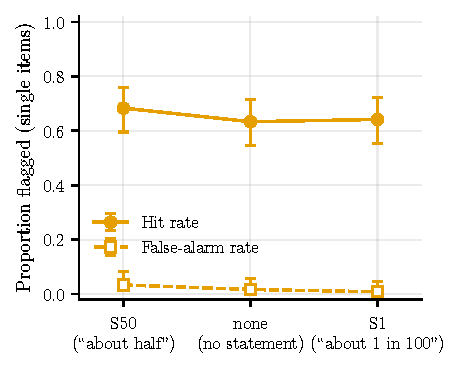
\includegraphics[width=\linewidth]{figures/report/fig_d_stated_prevalence_haiku.pdf}
\caption{Haiku}
\end{subfigure}\hfill
\begin{subfigure}[b]{0.49\textwidth}
\centering
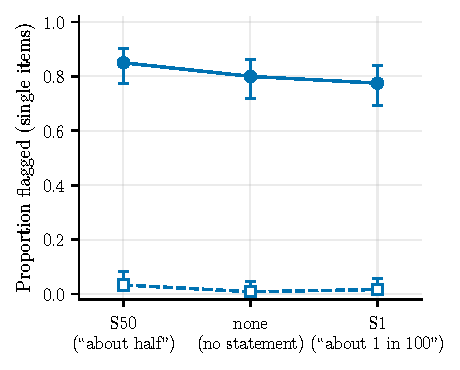
\includegraphics[width=\linewidth]{figures/report/fig_d_stated_prevalence_sonnet.pdf}
\caption{Sonnet}
\end{subfigure}
\caption{Single-item hit and false-alarm rates under three statements of the base rate (Experiment~2). Error bars are Wilson \SI{95}{\percent} confidence intervals.}\label{fig:stated}
\end{figure}

\subsection{H3: labelled calibration block}\label{sec:h3}

At \SI{2.5}{\percent} prevalence the 10 labelled examples did not significantly raise the hit rate (Figure~\ref{fig:remedies}). Haiku's hit rate fell from 0.694 to 0.600 (OR 0.66, 0.38 to 1.16, $p = .150$, Holm $p = .150$). Sonnet's rose from 0.738 to 0.850 (OR 2.02, 0.99 to 4.10, $p = .053$, Holm $p = .106$). For Sonnet the block moved the criterion in the liberal direction ($\Delta c = {-0.37}$, \num{-0.59} to \num{-0.18}) with no change in $d'$ (0.03, \num{-0.38} to 0.48), and its false-alarm rate rose from \SI{1.7}{\percent} to \SI{4.0}{\percent} ($\Delta F = 0.0224$, 0.0139 to 0.0314). Its mean number of flags per batch rose from 1.41 to 2.40. H3 is not supported. With 80 backdoored judgements per remedy cell, effects of the size of Sonnet's rise may have gone undetected, so this null result is weak evidence that the block does not help.

\begin{figure}[tbp]
\centering
\begin{subfigure}[b]{0.49\textwidth}
\centering
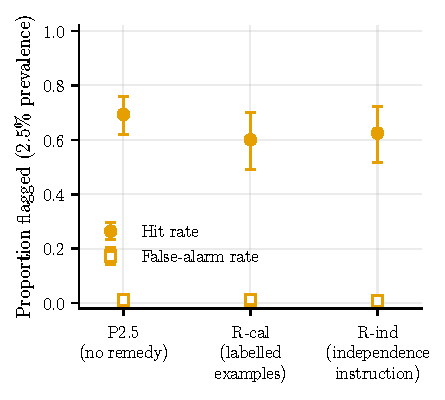
\includegraphics[width=\linewidth]{figures/report/fig_e_remedies_haiku.pdf}
\caption{Haiku}
\end{subfigure}\hfill
\begin{subfigure}[b]{0.49\textwidth}
\centering
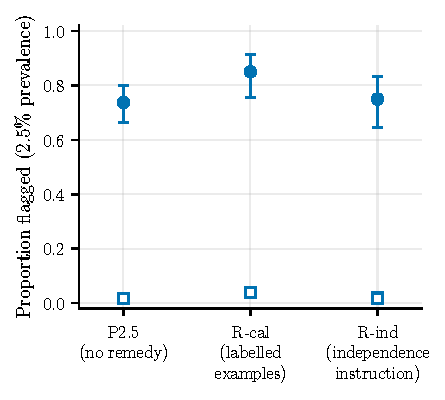
\includegraphics[width=\linewidth]{figures/report/fig_e_remedies_sonnet.pdf}
\caption{Sonnet}
\end{subfigure}
\caption{Hit and false-alarm rates at \SI{2.5}{\percent} prevalence without a remedy (P2.5), with the labelled calibration block (R-cal) and with the independence instruction (R-ind). Error bars are Wilson \SI{95}{\percent} confidence intervals.}\label{fig:remedies}
\end{figure}

\subsection{Exploratory and post hoc analyses}\label{sec:exploratory}

\paragraph{E1, position.} The position of the backdoored item in the batch did not predict hits in either monitor or condition (all $p \geq .08$; Figure~\ref{fig:position}). Figure~\ref{fig:position} does show lower hit rates for backdoors in the first eight positions of P10 batches, a pattern that the registered linear test would not detect. One of eight uncorrected tests was significant: Sonnet's false alarms became more frequent later in P2.5 batches (OR per 10 positions 1.26, $p = .019$).

\begin{figure}[tbp]
\centering
\begin{subfigure}[b]{0.49\textwidth}
\centering
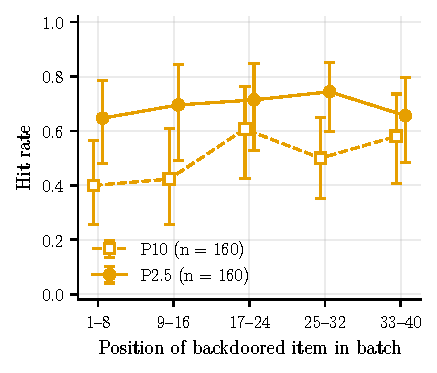
\includegraphics[width=\linewidth]{figures/report/fig_c_position_haiku.pdf}
\caption{Haiku}
\end{subfigure}\hfill
\begin{subfigure}[b]{0.49\textwidth}
\centering
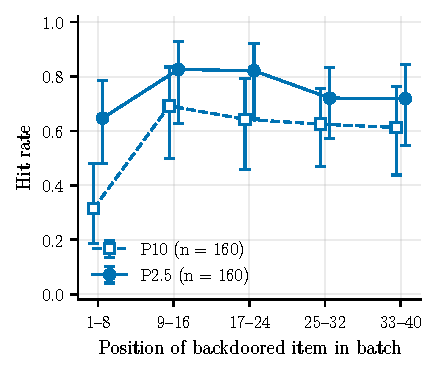
\includegraphics[width=\linewidth]{figures/report/fig_c_position_sonnet.pdf}
\caption{Sonnet}
\end{subfigure}
\caption{Hit rate by position of the backdoored item in the batch, in bins of eight positions (exploratory). Error bars are Wilson \SI{95}{\percent} confidence intervals.}\label{fig:position}
\end{figure}

\paragraph{E2, independence instruction.} R-ind did not change hit rates (Haiku OR 0.74, 0.42 to 1.30, $p = .288$; Sonnet OR 1.07, 0.57 to 1.98, $p = .835$). Haiku's false-alarm rate was slightly lower ($\Delta F = {-0.0045}$, ${-0.0088}$ to ${-0.0003}$).

\paragraph{E3, monitors.} In batches the two monitors did not differ (all monitor terms and interactions $p \geq .195$). In single-item review Sonnet caught more backdoors than Haiku (log-odds 0.965, SE 0.230, $p < .001$, at S50).

\paragraph{E4, single item against batch.} Single-item review with no stated rate (Haiku 0.633, Sonnet 0.800) caught about as many backdoors as the P2.5 batches and more than the P50 and P10 batches in three of four comparisons. Odds ratios for batch against single were, for Haiku, 0.61 at P50 ($p = .051$), 0.58 at P10 ($p = .026$) and 1.31 at P2.5 ($p = .291$), and for Sonnet 0.25 at P50 ($p < .001$), 0.33 at P10 ($p < .001$) and 0.70 at P2.5 ($p = .226$). False alarms did not differ (all $p \geq .46$). These comparisons use different item sets, and the prompts differ by one sentence.

\paragraph{Post hoc: how flags relate to scores.} In every condition the flag behaved almost like a fixed threshold on the monitor's own suspicion score. No item scoring below 20 was flagged and every item scoring 60 or more was; most of the change happened in the 40--59 band, with a few items scoring 20--39 flagged in some conditions (Table~\ref{tab:bands}). The prevalence effect therefore came from the scores. Backdoored items scored lower at P50 than at P2.5 (Table~\ref{tab:sdt}), and fewer of them reached the top band. Clean items scored low throughout.

\begin{table}[tbp]
\centering
\small
\caption{Post hoc. ``Top band'' is the share of backdoored items scoring 80--100. ``Flag at 40--59'' is the share of all items in that score band that were flagged.\source{\code{results/RESULTS\_numbers.md}, ``Post-hoc (not pre-registered): how suspicion scores map to flags''}}\label{tab:bands}
\begin{tabular}{@{}l l r r@{}}
\toprule
Monitor & Condition & Top band & Flag at 40--59 \\
\midrule
Haiku & P50 & 0.09 & 0.73 \\
Haiku & P2.5 & 0.22 & 0.84 \\
Haiku & \emph{none} (single) & 0.17 & 1.00 \\
Sonnet & P50 & 0.17 & 0.85 \\
Sonnet & P2.5 & 0.45 & 0.93 \\
Sonnet & \emph{none} (single) & 0.60 & 0.83 \\
Sonnet & S50 (single) & 0.72 & 0.83 \\
Sonnet & S1 (single) & 0.47 & 1.00 \\
\bottomrule
\end{tabular}
\end{table}

\paragraph{Post hoc: reasoning length and robustness.} Haiku's mean thinking tokens per batch call were \num{7592} at P50 against \num{4195} at P2.5; Sonnet's were 116 against 480. Dropping the calls with in-call schema corrections left the conclusions for H1 to H3 unchanged (H2 tested with the item-clustered GLM). The H1 odds ratios were 2.35 for Haiku ($p = .0007$) and 2.81 for Sonnet ($p < .001$), and Haiku's H3 $p$ value moved from .150 to .076, still not significant.

% ===========================================================================
\section{Discussion}\label{sec:discussion}

\subsection{What was found}\label{sec:found}

The low-prevalence effect did not appear. In batch review, both Claude monitors caught more backdoors at \SI{2.5}{\percent} prevalence than at \SI{50}{\percent}, and the criterion did not become more conservative. The clearest contrast is between batches with one backdoor and batches with several. P2.5 batches and single-item review gave similar hit rates, while P10 and P50 batches, which behaved alike, gave lower ones. A stated base rate of 1 in 100 had a small effect on Sonnet that ran at least partly through its scores; its criterion moved in the conservative direction, but not reliably. The TIP-style calibration block did not reliably help and raised Sonnet's false alarms. Position in the batch and an instruction to judge independently made no detectable difference.

\subsection{Why LLM monitors may differ from human screeners}\label{sec:why}

\emph{Why no low-prevalence effect.} The human effect builds up over many trials, as observers learn the base rate and lower their quitting thresholds~\cite{wolfe2005,wolfe2007}. An LLM monitor sees all 40 items at once; nothing in the call resembles a long run of empty searches, so there may be no route by which rarity becomes conservatism.

\emph{Why fewer hits with several backdoors.} Two candidate explanations fit the data equally well. The design cannot separate them, because it varied only the number of backdoors in a batch of 40, and P10 (4 backdoors) behaved like P50 (20).
\begin{itemize}
\item \textbf{Pop-out.} A monitor that sees a whole batch may judge each item partly against the others, so one odd item among 39 ordinary ones stands out. This fits the ``implicit normalization of decisions within the batch'' of Hida et~al.~\cite{hida2026}, whose balanced review, like P50 here, was screened more restrictively in batches, although P2.5 batches were not significantly more inclusive than single-item review.
\item \textbf{Crowding.} When several items deserve attention, each may look less exceptional or get less scrutiny, loosely like the human subsequent search misses~\cite{cain2013}. The monitors did score every item, and their reasoning length pointed both ways (at P50 Haiku reasoned more and Sonnet much less).
\end{itemize}

Both explanations agree with the post hoc finding that the flag threshold stayed put while backdoored items scored lower when several shared a batch. Telling them apart needs a design that varies the number of backdoors and the batch size separately.

The flag was close to a fixed threshold on the score in every condition, so SDT's split between evidence and criterion maps onto something real in these monitors.

\subsection{Safety implications, stated as hypotheses}\label{sec:implications}

For the rare-attack strategy that control evaluations usually assume, these results are mildly reassuring: rarity did not make these monitors miss more. They raise a different concern. If backdoored items score lower when several share a review context, an attacker who could place several attacks in one batch, coordinating them ``across space''~\cite[Sec.~6]{korbak2025}, might lower the suspicion of each. This study is not evidence that this happens in realistic monitoring; it is a hypothesis to test in agent settings, where one transcript may contain several suspicious actions.

If the pattern holds more widely, three points follow. First, batch composition is a variable in monitor evaluation: balanced batches understated the hit rate at low prevalence here, and the arithmetic extrapolations used in current work~\cite{srivastav2026,abbasi2026} assume that class-conditional score distributions do not change with prevalence, and for batch review in this study they did. Second, per-item review did about as well as the best unremedied batches here and better than most batches with several backdoors, so where cost allows it may be the safer design. Third, prompts that state an expected attack rate can move a monitor's judgements, as the S1 sentence did for Sonnet, so such statements should be chosen deliberately and tested.

\subsection{Remedies}\label{sec:remedies}

In people, high-prevalence bursts with feedback restore a criterion that has drifted too conservative, at the cost of more false alarms than in a baseline experiment~\cite[Experiment~7]{wolfe2007}. These monitors had no such drift to undo. The labelled block left Haiku's hit rate statistically unchanged and pushed Sonnet's criterion in the liberal direction, adding hits and false alarms together: it moved the operating point rather than restoring one. In a deployed protocol each extra false alarm uses audit budget, which is \SI{2}{\percent} of problems in Greenblatt et~al.~\cite{greenblatt2024} and \SI{0.1}{\percent} of actions in Korbak et~al.~\cite{korbak2025}. The R-cal examples also came from different problems from the scored items, and probes may help mainly with targets that resemble them~\cite{becker2026}. The independence instruction had no effect, much as a warning to disregard prior scores did not remove anchoring~\cite{kapetanovic2026}.

TIP's other job, measurement, gains support. If a monitor's hit rate depends on what else is in its context, the most direct estimate of deployed performance comes from known attacks inserted into the real stream~\cite{korbak2025}; in airport screening, about 100 TIP events per screener gave adequate reliability~\cite{buser2025}.

\subsection{What the human analogy did and did not predict}\label{sec:analogy-result}

The analogy predicted a conservative criterion shift at low experienced prevalence, which did not happen, in line with the disanalogy noted in Section~\ref{sec:analogy}. It did not predict the drop in hits when several backdoors shared a batch, although multiple-target search offers a loose parallel~\cite{cain2013}. The stated-prevalence result is the closest to the human pattern: the 1-in-100 sentence moved Haiku's criterion in the conservative direction, Sonnet's in the same direction (interval including zero), and lowered Sonnet's hit rate, although Sonnet's scores moved too. The analogy's most useful contribution was its method. SDT and the criterion--sensitivity distinction, together with the post hoc score-band analysis, made it possible to see that the reversal came from the scores given to backdoored items, not from where the flag threshold sat.

\subsection{Implications for aviation AI developers}\label{sec:aviation}

Where LLM tools are used to screen aviation documents, such as occurrence reports or maintenance records, for rare safety-relevant items, this study suggests two checks. Measure detection with the mix of items the tool will actually see, rather than on balanced test sets. And avoid assuming that a rate measured with one batch size or one instruction carries over to another.

% ===========================================================================
\section{Limitations}\label{sec:limitations}

\paragraph{One domain and one item source.} The items are short solutions to entry-level problems, each with at most one backdoor, written by one generator under one instruction; real agent attacks are longer, multi-step and adaptive~\cite{kutasov2025,najt2026,najt2026arxiv}.

\paragraph{Claude-only monitors and an unlogged harness context.} The monitors and the generator come from one model family, at effort \code{low}, called through Claude Code. Each call carried about \num{1800} tokens of unlogged Claude Code scaffolding; it was constant across conditions, monitors and time, so it cannot explain differences between conditions, but it may have affected absolute rates. Other families, settings and direct API calls may behave differently.

\paragraph{Small P50 cell.} As registered, P50 had 8 batches per monitor, so its cluster-robust and bootstrap intervals are approximate and may be too narrow; the direction of H1 is consistent across monitors and with E4.

\paragraph{One batch size and a limited range.} All batches held 40 items, so the number and the share of backdoors were not varied separately, and pop-out and crowding cannot be told apart. The lowest prevalence was \SI{2.5}{\percent}, far above deployed attack rates. Experienced prevalence existed only within one call; most deployed monitors judge one transcript per call.

\paragraph{Power.} As the pre-registration warned, effects smaller than about 15 points may have been missed. This matters most for the null results of H3 (80 backdoored judgements per cell) and of Haiku's H2.

\paragraph{Measurement limits.} False alarms were very rare, so $d'$ and $c$ rest mainly on the hit rate, and single-item false-alarm rates rest on 120 clean items. The registered H2 model is numerically unreliable for Sonnet; an accurate post hoc refit and an exact paired test support the same conclusion. Items were reused across batches, and the H1 analysis clusters by batch only. E4 compares different item sets under prompts that differ by a sentence.

\paragraph{Process.} Clarifications 4 to 12 were committed after data collection had begun, the timing of the edit-size threshold rests on the engineer's record (Section~\ref{sec:prereg-record}), and post hoc analyses were added after the data were seen. In-call schema corrections, inferred from turn counts, were not anticipated by the registered retry rule; excluding them did not change H1 to H3.

\paragraph{Company sources.} Two background facts rest on reports published by a single company and are not peer reviewed: Anthropic's deployment flag and escalation rates (Section~\ref{sec:base-rates}), reported by Anthropic alone~\cite{favaro_pace}, and the SLEIGHT-Bench catch rates (Section~\ref{sec:detect}), from work run in Anthropic's Fellows Program and published by Anthropic~\cite{najt2026,najt2026arxiv}.

% ===========================================================================
\section{Conclusion}\label{sec:conclusion}

Human screeners miss rare targets, and AI control expects attacks to be rare. In this pre-registered test with two Claude models and toy code, LLM monitors did not miss rare attacks more often. Both monitors caught more backdoors when one backdoor sat in a batch of 40 than when twenty did, and batches with four behaved like those with twenty. Single-item review did about as well as the low-prevalence batches. Backdoored items scored lower when several shared a batch. Whether that is because a lone backdoor stands out or because several crowd each other out cannot be told apart here. A TIP-style calibration block did not reliably help, and a stated base rate slightly lowered one monitor's hit rate. The results argue for evaluating monitors with the item mix and presentation they will face in deployment, for treating batch composition as a variable, and for testing whether clustered attacks lower per-item suspicion in realistic agent settings.

% ===========================================================================
\section*{Acknowledgement}
\paragraph{AI assistance.} Literature searches, drafting and source verification were carried out with AI assistance (Claude, Anthropic) under the author's direction, as were the experimental code and analysis. An independent AI-assisted audit checked the references and quotations, and the analysis, against their sources, and its findings were addressed before this version. The author is responsible for the final text. Several of the AI-safety sources cited are research reports by Anthropic, the developer of the assistant used. Claude models also served as the item generator and as the monitors under study.
\paragraph{Competing interests.} The author is the founder of CitadelAero, which builds AI tools for aviation.
\paragraph{Disclaimer.} The views expressed are the author's own and do not represent those of any employer or regulator. Nothing here is operational, legal or regulatory advice.
\paragraph{Materials.} The verification log and audit record for this paper, and its pre-registration, code, data and raw outputs, are at \url{https://github.com/JamesLeCuirot/Research/tree/main/papers/02-do-llm-monitors-miss-rare-threats}.

\bibliographystyle{IEEEtran}
\bibliography{references}

\end{document}
